\chapter{Systèmes hydrogénoïdes: structures fines et hyperfines}
\section{Équation de Schrödinger (rappel)}
	\begin{wrapfigure}[9]{r}{4cm}
	\vspace{-18mm}
	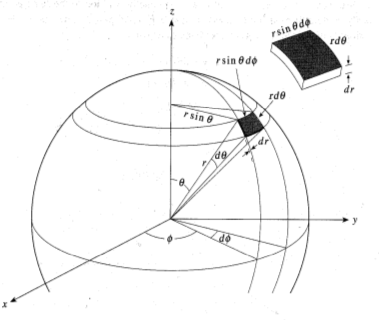
\includegraphics[scale=0.4]{ch1/image1}
	\captionof{figure}{ }
	\end{wrapfigure}
Avant toute chose, signalons que ce chapitre (ainsi que le suivant) est grandement inspiré
de \textit{Physics of Atomes and Molecules} de \textsc{B.H. Bransden} et \textsc{C.J.
Joachain}. Commençons par rappeler le système de coordonnées sphérique
\begin{equation}
\left\{\begin{array}{ll}
x &= r\sin\theta\cos\phi\\
y &= r\sin\theta\sin\phi\\
z &= r\cos\theta
\end{array}\right.
\end{equation}
Il convient de ne pas oublier le jacobien lors du changement de variable
\begin{equation}
d\vec{r} = dxdydz : (r\sin\theta d\phi)(rd\theta)dr = r^2\sin\theta drd\theta d\phi
\end{equation}

\subsection{Les harmoniques sphériques}
Le moment cinétique orbital $\vec{L}$ au carré s'écrit
\begin{equation}
\vec{L}^2 = \vec{L}.\vec L = L^2_x+L^2_y+L^2_z
\end{equation}
En coordonnée sphériques
\begin{equation}
\vec L^2 = -\hbar^2\left[\frac{1}{\sin\theta}\frac{\partial}{\partial \theta}\left(\sin\theta\frac{\partial}{
\partial \theta}\right)+\frac{1}{\sin^2\theta}\frac{\partial^2}{\partial\phi^2}\right]
\end{equation}
Les \textbf{harmoniques sphériques} sont par définition fonction propres de $\vec{L}^2$, mais aussi $L_z$\\

\cadre{\begin{equation}
\begin{array}{ll}
\vec{L}^2Y_{lm}(\theta,\phi) &= \hbar^2l(l+1)Y_{lm}(\theta,\phi)\\
L_z Y_{lm}(\theta,\phi) &= \hbar mY_{lm}(\theta,\phi)
\end{array}
\end{equation}
où $l=0,1,2,3,\dots$ et $m= l,l-1,l-2,\dots, -l$.}\ \\

Le choix de $m$ (pour \textit{magnétique}) prendra tout son sens lorsque l'on plongera le système dans un 
champ magnétique et que l'on perdra la symétrie sphérique par le fait qu'il existe une direction privilégiée. 
Comme ces deux observables ont des fonctions propres communes, elles doivent forcément commuter
\begin{equation}
[\vec{L}^2, L_z] = 0
\end{equation}
Pour nommer les orbitales, on donne un doux nom à chaque valeur de $l$\\

\cadre{$$l=0,1,2,3,4,5,6,7,\dots$$ $$s,p,d,f,h,i,k,\dots$$
où la lettre $j$ a volontairement été laissée sur le côté pour ne pas la confondre avec de $i$, ce qui 
pouvait facilement être le cas en utilisant des machines à écrire !}\ \\

Pour les retenir, un petit moyen mnémotechnique : \textit{"\textbf{S}olar \textbf{P}hysicists \textbf{D}on't
\textbf{F}ind \textbf{G}iraffes \textbf{H}idding \textbf{I}n \textbf{K}itchens}.\\

Les harmoniques sphériques sont définies pour $m \geq 0$ par 
\begin{equation}
Y_{lm} (\theta, \phi) = (-1)^m
\left[ \frac{(2l+1)}{4 \pi} \frac{(l-m)!}{(l+m)!}
\right] ^{\frac{1}{2}}  P^{m}_l (\cos \theta) e^{i m \phi}
\end{equation}
Dans le cas où $m$ est négatif, on trouve l'harmonique sphérique associée via : 
\begin{equation}
Y_{l,-m} (\theta, \phi) = (-1)^m Y^\ast_{lm} (\theta, \phi)
\end{equation}
Les harmoniques sphériques répondent aux relations d'orthonormalité, où il convient de ne pas oublier le 
facteur en $\theta$. Le prix à payer est bien évidemment celui de la normalisation :
\begin{equation}
\int_0^\pi d \theta \sin \theta 
\int_0^{2 \pi} d\phi \; Y_{lm}^\ast (\theta,\phi) \; 
Y_{l'm'} (\theta,\phi) = \delta_{ll'} \delta_{mm'}
\end{equation}

On peut définir des opérateurs de montée et de descente
\begin{equation}
L_+ \equiv L_x+iL_y,\qquad\qquad\qquad\qquad L_- \equiv L_x-iL_y
\end{equation}
Avec ceux-ci, il est possible de modifier la valeur de la projection du nombre quantique $l$, c'est-à-dire
$m_l$ (ou encore, $m$)
\begin{equation}
L_\pm Y_{lm}(\theta,\phi) = \hbar\sqrt{l(l+1)-m(m\pm 1)}Y_{lm\pm1}(\theta,\phi)
\end{equation}
\newpage
Suivant cette définition, voici quelques harmoniques sphériques 
\begin{equation}
\begin{array}{l}
 Y_{0,0} = \frac{1}{(4 \pi)^{1/2}}  \\
\ \\
 Y_{1,0} = \left( \frac{3}{4 \pi} \right)^{1/2} \cos \theta \\
 Y_{1,\pm 1}  = \mp \left( \frac{3}{8 \pi} \right)^{1/2} \sin \theta \; e^{\pm i \phi} \\
\ \\
 Y_{2,0} = \left( \frac{5}{16 \pi} \right)^{1/2} (3 \cos^2 \theta - 1)   \\
 Y_{2,\pm 1} = \mp \left( \frac{15}{8 \pi} \right)^{1/2} \sin \theta \cos \theta \; e^{\pm i \phi} \\
 Y_{2,\pm 2} = \left( \frac{15}{32 \pi} \right)^{1/2} \sin^2 \theta \; e^{\pm 2i \phi} \\
\ \\
 Y_{3,0} = \left( \frac{7}{16 \pi} \right)^{1/2}   (5 \cos^3 \theta - 3 \cos \theta)  \\
 Y_{3,\pm 1} = \mp \left( \frac{21}{64 \pi} \right)^{1/2}    \sin \theta (5 \cos^2 \theta - 1)  \; e^{\pm i \phi} \\
 Y_{3,\pm 2} =  \left( \frac{105}{32\pi} \right)^{1/2}    \sin^2 \theta \cos \theta \; e^{\pm 2 i \phi} \\
 Y_{3,\pm 3} = \mp \left( \frac{35}{64 \pi} \right)^{1/2}    \sin^3 \theta  \; e^{\pm 3 i \phi}
\end{array}
\end{equation}



\subsection{Les forces centrales}
Un potentiel central est un potentiel présentant une symétrie sphérique
\begin{equation}
V(\vec{r}) = V(r)
\end{equation}
où $r = |\vec r|$. Pour traiter ce potentiel de façon efficace, il convient d'écrire l'Hamiltonien 
\begin{equation}
H = -\frac{\hbar^2}{2m}\nabla^2+V(r)
\end{equation}
en coordonnées sphériques
\begin{equation}
H = -\frac{\hbar^2}{2m}\left[\frac{1}{r^2}\frac{\partial}{\partial r}\left(r^2\frac{\partial}{\partial r}\right)
+\frac{1}{r^2\sin\theta}\frac{\partial}{\partial \theta}\left(\sin\theta\frac{\partial}{\partial \theta}\right)
+ \frac{1}{r^2\sin^2\theta}\frac{\partial^2}{\partial \phi^2}\right] + V(r)
\end{equation}
En utilisant l'écriture sphérique de $\vec{L}^2$
\begin{equation}
\vec L^2 = -\hbar^2\left[\frac{1}{\sin\theta}\frac{\partial}{\partial \theta}\left(\sin\theta\frac{\partial}{
\partial \theta}\right)+\frac{1}{\sin^2\theta}\frac{\partial^2}{\partial\phi^2}\right]
\end{equation}
On peut écrire l'Hamiltonien sous une forme sphérique
\begin{equation}
H=-\frac{\hbar^2}{2m}\left[\frac{1}{r^2}\frac{\partial}{\partial r}\left(r^2\frac{\partial}{\partial r}\right)
-\frac{\vec L^2}{\hbar^2 r^2}\right] + V(r)
\end{equation}
Cet Hamiltonien vérifie les relations de commutation suivante
\begin{equation}
[H,\vec{L}^2] = [H,L_z] = [\vec{L}^2,L_z] = 0
\end{equation}
Il est possible de résoudre l'équation de Schrödinger par la méthode de séparation des variables, à l'aide
de nos harmoniques sphériques
\begin{equation}
\psi_{E,l,m}(r,\theta,\phi) = R_{E,l}(r)Y_{lm}(\theta,\phi)
\end{equation}
On peut alors obtenir l'équation radiale
\begin{equation}
\left\{-\frac{\hbar^2}{2m}\left[\frac{1}{r^2}\frac{d}{dr}\left(r^2\frac{d}{dr}\right) - \frac{l(l+1)}{r^2}\right]+
V(r)\right\}R_{E,l}(r) = ER_{E,l}(r)
\end{equation}
En effectuant le changement de variable $P_{E,l}(r) \equiv rR_{E,l}(r)$, on retrouve une équation de 
Schrödinger sous un format "classique"
\begin{equation}
\left[-\frac{\hbar^2}{2m}\frac{d^2}{dr^2}+\frac{\hbar^2l(l+1)}{2mr^2}+V(r)\right]P_{E,l}(r) = EP_{E,l}(r)
\end{equation}
On retiendra le comportement asymptotique suivant, pour $r\to0$ : $P_{E,l}(r) \sim r^{l+1}$.\\


La fonction factorisée $\psi_{E,l,m}(r,\theta,\phi) = R_{E,l}(r)Y_{lm}(\theta,\phi)$ respecte les règles 
d'inversion et de parité. On défini l'opération d'inversion (ou parité)
\begin{equation}
I\psi_{E,l,m}(\vec{r}) = I\psi_{E,l,m}(-\vec{r})
\end{equation}
Comme $I = I^\dagger$, ses valeurs propres sont réelles. Grâce à sa commutation avec l'Hamiltonien, on peut
écrire
\begin{equation}
[H,I]=0\Rightarrow I\psi_{E,l,m}(r)=\alpha\psi_{E,l,m}(r)
\end{equation}
Comme $I^2=E$, il en vient que $\alpha^2$ est forcément l'unité. Dès lors, $\alpha = \pm1$. Ceci revient à 
effectuer le changement de variable suivant (en cartésien et sphérique)
\begin{equation}
\left\{\begin{array}{ll}
x &\to -x\\
y &\to -y\\
z &\to -z
\end{array}\right. \qquad\qquad\qquad\left\{\begin{array}{ll}
r &\to -r\\
\theta &\to (\pi-\theta)\\
\phi &\to (\phi+\pi)
\end{array}\right. 
\end{equation}
Appliquons cet opérateur sur notre fonction factorisée :$I\psi_{E,l,m}(r,\theta,\phi) = I[R_{E,l}(r)Y_{lm}(\theta,
\phi)]$. Ceci donne
\begin{equation}
I\psi_{E,l,m}(r,\theta,\phi) = R_{E,l}(r)[IY_{lm}(\theta,\phi)] = (-1)^lR_{E,l}(r)Y_{lm}(\theta,\phi)
\end{equation}
où l'on voit apparaître la fonction factorisée. Nous avons ainsi défini l'effet de l'application de l'opérateur
parité sur la fonction d'onde \\

\cadre{
\begin{equation}
I\psi_{E,l,m}(r,\theta,\phi) = (-1)^l\psi_{E,l,m}(r,\theta,\phi)
\end{equation}}\ \\

Ainsi, $l$ pair implique $\alpha=+1$ et l'on parlera d'états \textbf{pairs}. A l'inverse, on parlera d'états
\textbf{impairs}.




\subsection{Problème à 2 corps: effet de masse}
Considérons deux particules en interaction
\begin{equation}
H = \frac{\vec p_1^2}{2m_1}+\frac{\vec p_2^2}{2m_2}+V(\vec r_1-\vec r_2)
\end{equation}
A l'aide du principe de correspondance $p\to -i\hbar\vec\nabla$ et $\vec{L}\to \vec{L}=-i\hbar(\vec{r}\times
\vec\nabla)$, on peut retrouver l'équation de Schrödinger
\begin{equation}
i\hbar\frac{\partial}{\partial t}\Psi(\vec{r}_1,\vec{r}_2, t) = \left[-\frac{\hbar^2}{2m_1}\nabla_1^2
-\frac{\hbar^2}{2m_2}\nabla_2^2+V(\vec r_1-\vec r_2)\right]\Psi(\vec{r}_1,\vec{r}_2, t)
\end{equation}
où $V$ ne dépend que de la coordonnée relative $\vec{r} =\vec{r_1}-\vec{r_2}$. Il est également pratique 
d'exprimer la coordonnée relative du centre de masse $\vec{R} = \frac{m_1\vec r_1+m_2\vec r_2}{m_1+m_2}$.
Effectuons alors le changement de coordonnées $(\vec{r_1},\vec{r_2})\to (\vec{r},\vec{R})$. Ceci peut se 
faire en définissant la masse totale et la masse réduite
\begin{equation}
M=m_1+m_2,\qquad\qquad\qquad \mu = \frac{m_1m_2}{m_1+m_2}
\end{equation}
En définissant le moment relatif $\vec{p}=\frac{m_2\vec p_1-m_1\vec p_2}{m_1+m_2}$ et le moment total $\vec{P}
= \vec{p_1}+\vec{p_2}$, nous avons que
\begin{equation}
\frac{\vec p_1^2}{2m_1}+\frac{\vec p_2^2}{2m_2} = \frac{\vec P^2}{2M}+\frac{\vec p^2}{2\mu}
\end{equation}
L'équation de Schrödinger devient
\begin{equation}
i\hbar\frac{\partial}{\partial t}\Psi(\vec R, \vec r, t) = \left[-\frac{\hbar^2}{2M}\nabla_R^2
-\frac{\hbar^2}{2\mu}\nabla_r^2+V(\vec r)\right]\Psi(\vec R, \vec r, t)
\end{equation}
où l'on voit cette fois-ci clairement apparaître la masse réduite $\mu$. Lorsque le potentiel $V$ est 
indépendant du temps $t$, il est possible d'effectuer le découplage du centre de masse et du mouvement 
relatif
\begin{equation}
\Psi(\vec R, \vec r, t) = \Phi(\vec{R})\psi(\vec{r})e^{-i(E_{CM}+E)t/\hbar}
\end{equation}
Ce découplage implique que l'on considère une particule libre de masse $M$ pour le centre de masse
\begin{equation}
-\frac{\hbar^2}{2M}\Delta_R^2\Phi(\vec{R}) = E_{CM}\Phi(\vec{R})
\end{equation}
Nous avons également à considérer une particule de masse $\mu$, cette fois-ci dans un potentiel $V(r)$
\begin{equation}
\left[-\frac{\hbar^2}{2\mu}\nabla_r^2+V(r)\right]\psi(\vec{r}) = E\psi(\vec{r})
\end{equation}
où nous retrouvons bien la masse réduite. Dans le contexte de l'atome d'hydrogène, celle-ci sera proche de la
masse de l'électron. \\

L'énergie totale à considérée est bien donnée par
\begin{equation}
E_{tot} = E_{CM}+E
\end{equation}


\subsection{Systèmes hydrogénoïdes – Potentiel de Coulomb}
Pour un système hydrogénoïde, nous devons utiliser l'équation décrivant le mouvement relatif
\begin{equation}
\left[-\frac{\hbar^2}{2\mu}\nabla_r^2+V(r)\right]\psi(\vec{r}) = E\psi(\vec{r})
\end{equation}
En utilisant comme potentiel le potentiel de \textsc{Coulomb} (potentiel central)
\begin{equation}
V(\vec{r}) = V(r) = -\dfrac{Ze^2}{4\pi\epsilon_0r}
\end{equation}
Celui-ci est le reflet d'un potentiel liant (négatif, ceci reflétant de \textsc{Coulomb} liant deux charges
opposées).

Cherchons les solutions en coordonnées sphérique $\psi_{E,l,m}(r,\theta,\phi) = R_{E,l}(r)Y_{lm}(\theta,\phi)$. 
L'équation radiale s'écrit
\begin{equation}
\left\{-\frac{\hbar^2}{2\mu}\left[\frac{1}{r^2}\frac{d}{dr}\left(r^2\frac{d}{dr}\right) - \frac{l(l+1)}{r^2}\right]+
V(r)\right\}R_{E,l}(r) = ER_{E,l}(r)
\end{equation}
où $r$ est la coordonnées relative et où ce n'est pas la masse de l'électron $m$ qui apparaît mais la masse
réduite $\mu$. C'est l'effet de masse qui apparaît lorsque les choses sont traitées correctement. Avec le 
changement de variable $P_{E,l}(r) \equiv rE_{E,l}(r)$ et en substituant , on trouve\\

\cadre{
\begin{equation}
\left[-\frac{\hbar^2}{2\mu}\frac{d^2}{dr^2}+\frac{\hbar^2l(l+1)}{2\mu r^2}-\frac{Ze^2}{4\pi\epsilon_0r}\right]P_{E,l}(r) = EP_{E,l}(r)
\end{equation}
\danger\ C'est bien la masse réduite $\mu$ qui apparaît ici.}\ \\

Cette équation permet de décrire les systèmes hydrogénoïdes, c'est-à-dire les systèmes atomiques à un seul
électron ($Z=1 : H, Z=2 : He^+, Z=91 :\  ^{91}U^{90+}, \dots$).\\


	\begin{wrapfigure}[14]{r}{4cm}
	\vspace{-5mm}
	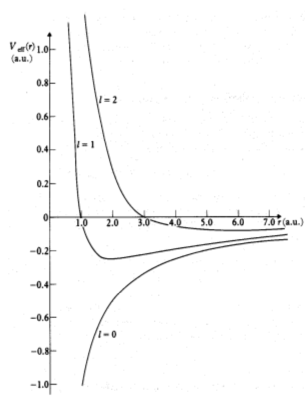
\includegraphics[scale=0.4]{ch1/image2}
	\captionof{figure}{ }
	\end{wrapfigure}
Pour retrouver une équation de Schrödinger "classique", on définit le \textit{potentiel effectif} $V_{eff}^{(l)}$
\begin{equation}
V_{eff}^{(l)} = -\frac{Ze^2}{4\pi\epsilon_0r}+\dfrac{l(l+1)\hbar^2}{2\mu r^2}
\end{equation}
Le second terme du membre de droite est le \textit{potentiel centrifuge} qui, contrairement au potentiel
de \textsc{Coulomb}, est antiliant (signe positif). Le potentiel effectif est déterminé par la valeur de
$l$ : une valeur nulle de $l$ donne le potentiel coulombien.\\

Cependant, dès que $l\neq 0$, une nouvelle contribution à petite distance apparaît. Elle relève l'existence d'un
potentiel centrifuge qui fait que l'on a une barrière coulombienne que l'on ne retrouve pas pour $l=0$. Ceci
explique le comportement différent pour un électron $s$ ou $p$, le potentiel étant totalement différent.


\newpage
\subsection{Solution pour les états liés}
La solution de l'équation ci-dessus pour des états liés est donnée par 
\begin{equation}
E_n = -\frac{1}{2n^2}\left(\frac{Ze^2}{4\pi\epsilon_0}\right)^2\frac{\mu}{\hbar^2}=-\frac{e^2}{(4\pi\epsilon_0)
a_0}\left(\frac{\mu}{m}\right)\frac{Z^2}{2n^2}
\end{equation}
où $a_0=\frac{(4\pi\epsilon_0)\hbar^2}{me_2}$ est le rayon de \textsc{Bohr}.\\

	\begin{wrapfigure}[23]{l}{8.5cm}
	\vspace{-5mm}
	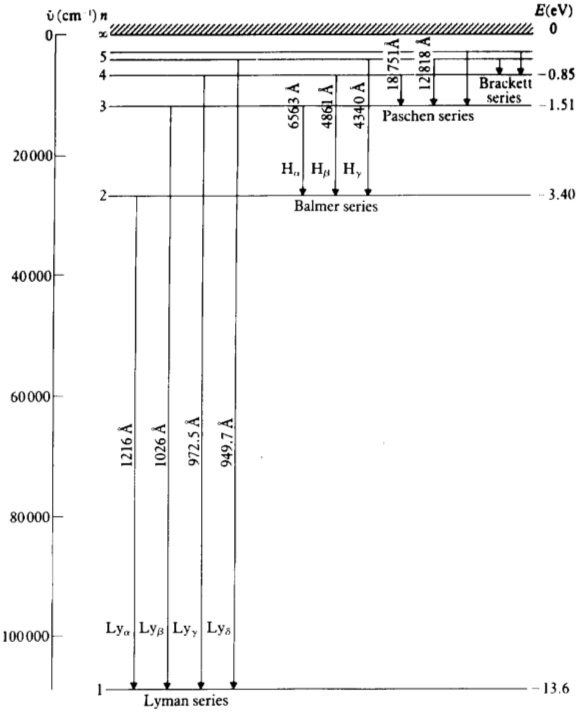
\includegraphics[scale=0.4]{ch1/image3}
	\captionof{figure}{ }
	\end{wrapfigure}
	
	Ci-contre, la représentation de la solution pour les états liés dans le cadre de l'atome d'hydrogène
	($Z=1, \mu=m$). La première chose que l'on peut constater est la présence de transition dans quasi toutes
	les classes, tout dépend de la transition regardées. On retrouve les raies de \textsc{Lyman} (transitions
	vers $n=1$), les raies de \textsc{Balmer} (transitions vers $n=2$), les raies de \textsc{Paschen}
	(transitions vers $n=3$) mais également les raies de \textsc{Brackett} (transitions vers $n=4$).\\
	
	Pour l'état $n=2$, on retrouve les états $2s_0, 2p_{+1}$ et $2p_{-1}$ qui sont tous caractérisés par
	une énergie $E_2$ donnée par la solution ci-dessus. Le niveau fondamental (énergie de 13.6 eV) n'est 
	autre que l'état $1s$. On note souvent les énergie en $cm^{-1}$, d'où l'échelle verticale. Si on regarde
	la différence entre $n=2$ et $n=1$, elle vaut à peu près $100'000$ cm$^{-1}$. Il s'agit du \textbf{
	nombre d'onde} défini comme l'inverse de la longueur d'onde. Plusieurs écritures sont possibles
	\begin{equation}
	\frac{1}{\lambda}\equiv \bar\lambda = \sigma = \bar\nu
	\end{equation}
	La longueur d'onde est l'inverse de cette "distance" et on retrouve bien la valeur de 1216 Angström. 
	Il existe une relation donnant la fréquence en fonction de la différence de l'inverse de deux nombres 
	entiers multipliée par une certaine constante afin que ce soit correction dimensionnement
	\begin{equation}
	\nu = R_\infty\left(\frac{1}{n_1^2}-\frac{1}{n_2^2}\right)\qquad\text{où }\quad R_\infty = \frac{m}{
	4\pi\hbar^3}\left(\frac{e^2}{4\pi\epsilon_0}\right)^2
	\end{equation}
	

\subsection{Système d'unités atomiques}
Le système d'unité atomique est un système horrible ou tout vaut 1. Avant de l'énoncer, rappelons la 
définition du rayon de \textsc{Bohr}
\begin{equation}
a_0=\frac{(4\pi\epsilon_0)\hbar^2}{me_2} = 5.29\times 10^{-11}\text{ m}
\end{equation}
On dira que $a_0$ = 1 u.a. de longueur. Si on veut savoir, ce que ça vaut, il faudra faire les bonnes
substitution dans la formule de $a_0$ sachant que
$m=m_e$ = 1 u.a. de masse, $e$ = 1 u.a. de charge, $\hbar$ = 1 u.a. de moment angulaire et $4\pi\epsilon_0$ =
1 u.a.  de permittivité du vide. Ce choix d'unité est fait pour déterminer avec intelligence l'énergie. Si on 
évalue l'énergie $E_n$ ci-dessus avec ces unités, presque tout va se simplifier.\\

Sachant que une unité atomique d'énergie est donnée par $E_h = e^2/(4\pi\epsilon_0 a_0)$, il est vient que
$E_n \approx -\frac{Z^2}{2n^2}E_h$. Pour $Z=1$, on trouve $E_{n=1} \approx -1/2 E_h$. Il est possible de 
retrouver la valeur sachant que $1 E_h$ (un hartree) vaut 27.2 eV.\\

Ce système simplifie également les vitesses
\begin{equation}
v_0 = \frac{e^2}{(4\pi\epsilon_0)\hbar}\equiv \alpha c = 1 \text{ u.a. de vitesse}
\end{equation}
Comme $\alpha \approx 1/137$, on en déduit que $c\approx 137$ u.a. de vitesse.\\


\subsection{Solutions pour les états liés}
Compte tenu de ce système d'unité, on peut alors ré-écrire la solution pour les états liés d'énergie $E_n$
\begin{equation}
E_n = -\frac{e^2}{(4\pi\epsilon_0)a_\mu}\frac{Z^2}{2n^2}=-\dfrac{Z^2}{2n^2}\left(\frac{\mu}{m}\right)\text{ u.a.}
\end{equation}
La fonction radiale s'écrit alors
\begin{equation}
R_{nl}(r) = P_{nl}(r) / r=
  - \left\{ \left( \frac{2Z}{na_\mu} \right)^3
   \frac{(n-l-1)!}{2n[(n+l)!]^3} \right\}^{1/2} \;
  e^{-\rho/2} \rho^l \; L^{2l+1}_{n+l} (\rho)
\end{equation}
$\mbox{o\`u}~L^{2l+1}_{n+l}(\rho)~\mbox{est un polyn\^ome de
degr\'e}~n_r = n-l-1$. On possède donc une loi d'échelle reliant $\rho$ à $r$.
\begin{equation}
\rho 
= \frac{2Z}{na_\mu} \; r, \hspace*{2cm} 
 a_\mu = \frac{4 \pi \epsilon_0 \hbar^2}{\mu e^2}
\end{equation}
Quelques exemples, pour le plaisir des yeux
\begin{equation}
\begin{array}{l}
R_{10}(r) = 2 (Z/a_0)^{3/2} \exp (-Zr/a_0) \\
\ \\
R_{20}(r) = 2 (Z/2 a_0)^{3/2} (1-Zr/2 a_0) \exp (-Zr/2 a_0) \\
R_{21}(r) = \frac{1}{\sqrt{3}}  (Z/2 a_0)^{3/2} (Zr/a_0)
        \exp (-Zr/2 a_0) \\
\ \\
R_{30}(r) = 2 (Z/3a_0)^{3/2} (1 - 2Zr/3 a_0 + 2 Z^2r^2/27a_0^2) \\
  \hspace*{4cm}  \exp(-Zr/3a_0) \\
R_{31}(r) = \frac{4 \sqrt{2}}{9} (Z/3a_0)^{3/2}
  (1 -Zr/6a_0)(Zr/a_0) \\
  \hspace*{4cm} \exp(-Zr/3 a_0) \\
R_{32}(r) = \frac{4}{27 \sqrt{10}} (Z/3a_0)^{3/2} (Zr/a_0)^2 
   \exp(-Zr/3a_0)
\end{array}
\end{equation}
Notons que le nombre de nœuds est donné 
par $n_r=n-l-1$.

\subsubsection{Densités radiales}
Le \textit{slide 19} donne des exemples de densité radiale, justifiant la structure en couche des 
électrons et orbitales dans les systèmes polyélectroniques. On remarque que lorsqu'il y a deux nœuds 
radiaux, on les retrouve dans la structure en densité (qui s'annule la où la fonction radiale s'annule). Elles
sont forcément positives car elle détermineront les densités de probabilités.\\

On remarque que $2s$ s'éteint de façon exponentielle, sans nœud. La grande différence entre l'orbitale $s$ et
les autres est qu'elle est non-nulle en $r=0$ (car pas de potentiel centrifuge).


\section{Spectre de l’atome d’hydrogène}

\subsection{Série de Balmer}
	\begin{wrapfigure}[12]{l}{8cm}
	\vspace{-5mm}
	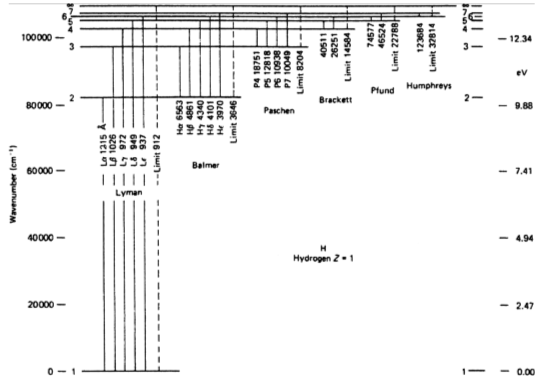
\includegraphics[scale=0.4]{ch1/image4}
	\captionof{figure}{ }
	\end{wrapfigure}
\textsc{Balmer} a observé une série de raie qui convergent vers une certaine limite, l'ionisation. Ainsi, la
raie qui a la plus proche longueur d'onde se rapproche de l'ionisation (il s'agit donc de la plus grande 
transition de \textsc{Balmer} en nombre de cm$^{-1}$ sur le spectre vu précédemment). Le spectre (version 
nombre d'onde $1/\lambda$) peut s'obtenir via
\begin{equation}
\tilde{\nu} = \tilde{R}\left(\frac{1}{n_1^2}-\frac{1}{n_2^2}\right)
\end{equation}
où $\tilde{R}_H = 109\ 677.58\ \text{cm}^{-1}$.\\

En fixant $n_1$ ($< n_1$) et en faisant flotter $n_2$ on peut retrouver les séries de
\begin{multicols}{2}
\begin{description}
\item[Lyman] $n_1=1$, UV
\item[Balmer] $n_1=2$, visible
\item[Paschen] $n_1=3$, IR
\item[Brackett] $n_1=4$, IR (lointain)
\item[Pfund] $n_1=5$, IR (très lointain)
\item[Hymphreys] $n_1=6$, IR (presque radio)
\end{description}
\end{multicols}


\subsection{Règle de Laporte et nomenclature}
	\begin{wrapfigure}[13]{r}{5.5cm}
	\vspace{-5mm}
	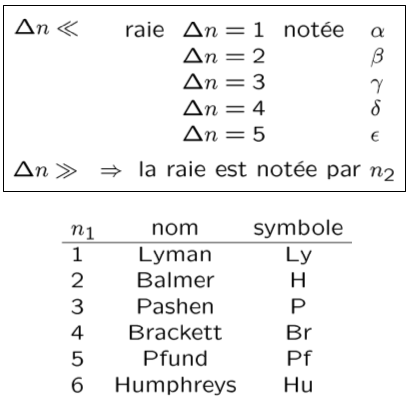
\includegraphics[scale=0.4]{ch1/image5}
	\captionof{figure}{ }
	\end{wrapfigure}
Il s'agit d'une représentation proposée par \textsc{Grotrian}. Celle-ci se base sur une représentation des
ensemble des niveaux avec les transitions permises et les règles de sélection. La règle de \textsc{Laporte} 
(Règle de sélection ($E1$) : $\Delta l = \pm 1$). sera approfondie au chapitre 3. \\

Le nombre d'onde s'exprime
\begin{equation}
\bar \nu = \frac{1}{\lambda} = \frac{1}{hc}(E_{n_1}-E_{n_2}) = \bar R_H\left(\frac{1}{n^2_1}-\frac{1}{n^2_2}
\right)
\end{equation}
On définit également
\begin{equation}
\bar{R}_H = \frac{\mu}{m_e}\bar{R}_\infty = \left(\frac{M_H}{M_H+m_e}\right)\bar{R}_\infty
\end{equation}
où $\bar{R}_H = 109677.581$ cm$^{-1}$ et $\bar{R}_\infty = 109737.31$ cm$^{-1}$.



\subsection{Effet de masse : Hydrogène et Deutérium}
Dans le spectre d'émission de l'hydrogène, on remarque que l'on a une raie très proche aux alentours de la
première raie (la plus à gauche)\footnote{Juste à côté de $H\alpha$ (voir nomenclature), on devine la présence
d'une autre raie : c'est celle du deutérium.}. Calculons l'émission de $H\alpha$
\begin{equation}
\bar\nu = \frac{1}{\lambda}= \bar{R}_H\left(\frac{1}{4}-\frac{1}{9}\right) = 15237\ \text{cm}^{-1}
\end{equation}


	\begin{wrapfigure}[14]{l}{6cm}
	%\vspace{-5mm}
	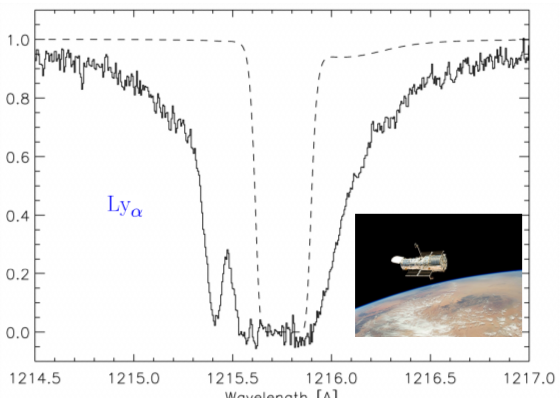
\includegraphics[scale=0.3]{ch1/image6}
	\captionof{figure}{On remarque un \textit{pic de deutérium} sur la \textsc{Lyman}$\alpha$. Elle se 
	situe dans l'UV (longueur d'onde plus petite que celle de l'hydrogène).}
	\end{wrapfigure}
Sachant que\footnote{Revoir le sens de $R$. D'où ça sort?} pour le deutérium $R_D = \frac{\mu_D}{\mu_H}R_H$ 
et connaissant $M_H$ et $M_D$, on peut évaluer le rapport des deux
\begin{equation}
\frac{\mu_D}{\mu_H} = \left(\frac{M_H+m_e}{M_Hm_e}\right)\left(\frac{M_Dm_e}{M_D+m_e}\right)=1.00027
\end{equation}
Il y a émission $H\alpha$ dans le deutérium à 15233 cm$^{-1}$. Il faut donc une très bonne résolution pour
pouvoir l'observer : il s'agit d'un effet plus fin que la structure fine. On définit le \textit{rapport 
d'abondances cosmiques}
\begin{equation}
\frac{[D]}{[H]}=2\times 10^{-5}
\end{equation}
Ceci signifie que les raies de l'hydrogène seront souvent \textit{optically thick} si celle de $D$ sont 
observables.

\section{Spectre des systèmes hydrogénoïdes}
\subsection{Loi d'échelle}
	\begin{wrapfigure}[8]{r}{6cm}
	\vspace{-8mm}
	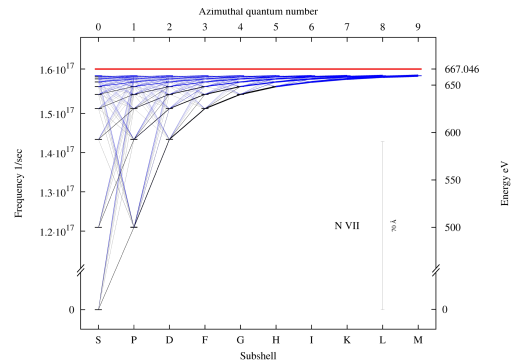
\includegraphics[scale=0.35]{ch1/image7}
	\captionof{figure}{ }
	\end{wrapfigure}
L'azote sept (en lettre grecques, $N\ VII$ ou $N^{6+}$ ($Z=7$)) est le septième spectre de l'azote. Il
est hydrogénoïde car bien qu'il possède sept protons, il n'a qu'un seul électron. On remarque que 
\begin{equation}
\begin{array}{lll}
E_n &=\DS -\frac{1}{2n^2}\left(\frac{Ze^2}{4\pi\epsilon_0}\right)^2\frac{m_e}{\hbar^2}\qquad \ &\propto
 Z^2\vspace{2mm}\\
I_P &=\DS \frac{1}{2}\frac{m_e}{\hbar^2}\left(\frac{Ze^2}{4\pi\epsilon_0}\right)^2 &=13.6\ Z^2\ \text{eV}
\end{array}
\end{equation}
On voit ainsi un effet liant de la charge sur le spectre (la proportionnalité en $Z^2$). Plus $Z$ augmente, 
plus $\bar R_M$ tend vers $\bar R_\infty = 109\ 737.32$. En effet, plus $Z$ augmente plus les niveaux sont
écartés mais plus la longueur d'onde diminue (évolue en $Z^{-2}$). Cette augmentation de $Z$ causant une 
diminution de $\lambda$ et une augmentation de $\bar R_M$ implique que le seul électron restant est 
"de plus en plus léger". La correction de masse est donc d'autant plus grande que le noyau est léger.\\

Il faut également prendre en compte les effets relativiste. Connaissant la vitesse de l'électron dans 
la première orbite de \textsc{Bohr}, on peut établir le rapport suivant
\begin{equation}
\frac{v}{c} = \alpha Z \approx \frac{Z}{137}
\end{equation}
Si $Z$ est faible, on peut négliger les effets relativiste. Par contre, si $Z$ est de l'ordre de 100, cela
signifie que la vitesse de l'électron est plus élevée : il va falloir prendre en compte les effets 
relativites. La vitesse de l'électron est ainsi d'autant plus grande que le nombre de proton est élevé. 
Passé un certain nombre, il faudra passer en relativiste et utiliser \textsc{Dirac} et non plus
\textsc{Schrödinger}\footnote{Pour un $Z$ grand, même dans un système hydrogénoïde, il faudra tenir compte
des effets relativiste. Notons qu'il n'y a pas de contradiction pour $Z>137$ (c'est bien possible) . Il 
faut en effet se rappeler que la vitesse de l'électron est estimée d'un modèle non-relativite.}.


\section{Le spin électronique}
\subsection{Les matrices de Pauli}
Pour un fermions, nous avons 
\begin{equation}
\left\{\begin{array}{ll}
s &= 1/2\\
m_s &= +s, \dots, -s \Rightarrow m_s = \pm 1/2
\end{array}\right.\qquad\qquad\left\{\begin{array}{ll}
\left[S_x,S_y\right] &= i\hbar S_z\\
\left[S_y,S_z\right] &= i\hbar S_x\\
\left[S_z,S_x\right] &= i\hbar S_y
\end{array}\right.
\end{equation}
Comme $\vec{S}^2$ et $S_z$ commutent, il existe un \textsc{ecoc} de ces deux observables
\begin{equation}
[\vec{S}^2, S_z] = 0\Rightarrow \{\vec{S}^2, S_z\} \text{ forme un \textsc{ecoc}}
\end{equation}
Il existe donc une base de fonctions propres communes :
\begin{equation}
\left\{\begin{array}{ll}
\vec{S}^2 \chi_{s,m_s} &= s(s+1)\hbar^2\chi_{s,m_s}\\
S_z\chi_{s,m_s} &= \hbar m_s\chi_{s,m_s}
\end{array}\right.
\end{equation}
Nous allons adopter la notation suivante 
\begin{equation}
\left\{\begin{array}{ll}
\alpha &\equiv \chi_{1/2,1/2}\\
\beta &\equiv \chi_{1/2,-1/2}
\end{array}\right.
\end{equation}
Ceci nous permet de faire la différence entre spin \textit{up} et \textit{down} en fonction de la valeur
propre de $S_z$.
\begin{equation}
\begin{array}{ll}
\text{spin \textbf{up}}\ \uparrow\\
\vec{S}^2\alpha &= (3/4)\hbar^2\alpha\\
S_z\alpha &= +(1/2)\hbar \alpha
\end{array}\qquad\qquad\qquad
\begin{array}{ll}
\text{spin \textbf{down}}\ \downarrow\\
\vec{S}^2\alpha &= (3/4)\hbar^2\alpha\\
S_z\alpha &= -(1/2)\hbar \alpha
\end{array}
\end{equation}

On peut écrire une fonction d'onde avec \textit{un peu de spin up et un peu de spin down}
\begin{equation}
\chi = \chi_+\alpha+\chi_-\beta
\end{equation}
où
\begin{equation}
\begin{array}{lll}
\bra{\alpha}\ket{\alpha} &= \bra{\beta}\ket{\beta} &= 1\\
\bra{\alpha}\ket{\beta} &= \bra{\beta}\ket{\alpha} &= 0
\end{array}\quad\Rightarrow\quad |\chi_+|^2+|\chi_-|^2=1
\end{equation}
Nous allons travailler dans un espace bidimensionnelle sous-tendu par les vecteurs \textit{purement up} et 
\textit{purement down}
\begin{equation}
\alpha = \left(\begin{array}{c}
1\\
0
\end{array}\right),\qquad\qquad\qquad\beta = \left(\begin{array}{c}
0\\
1
\end{array}\right)
\end{equation}
De même dans l'espace dual en considérant l'adjoint
\begin{equation}
\alpha^\dagger = (1\ 0), \qquad\qquad\qquad \beta^\dagger = (0\ 1)
\end{equation}
On peut jouer avec les opérateurs de montée et de descente
\begin{equation}
S_\pm \equiv S_x \pm i S_y
\end{equation}
On peut montrer que l'on ne monde pas un spin \textit{up} mais aussi que l'on ne descend pas un spin \textit{down}
\begin{equation}
S_+\alpha = 0,\qquad\qquad S_-\alpha = \hbar\beta,\qquad\qquad S_+\beta = \hbar\alpha,\qquad\qquad S_-\beta = 0
\end{equation}
Le vecteur $S_z$ lève l'ambiguïté rencontrée avec $\vec S^2$. Dans les représentations de l'espace 2D sous-tendu
à ces vecteurs, $S_+$ et $S_-$ sont bien évidemment orthogonaux. Il est possible de les écrire sous forme
matricielle
\begin{equation}
\vec{S}^2 = \frac{3}{4}\hbar^2\left(\begin{array}{cc}
1&0\\
0&1
\end{array}\right),\quad 
S_z = \frac{\hbar}{2}\left(\begin{array}{cc}
1&0\\
0&-1
\end{array}\right),\quad
S_+ = \hbar\left(\begin{array}{cc}
0&1\\
0&0
\end{array}\right),\quad S_- = \hbar\left(\begin{array}{cc}
0&0\\
1&0
\end{array}\right)
\end{equation}
Ces expressions nous permettent d'écrire $S_x$ et $S_y$ de façon matricielle
\begin{equation}
S_x = \left(\begin{array}{cc}
0&1\\
1&0
\end{array}\right),\qquad\qquad
S_y = \left(\begin{array}{cc}
0&-i\\
i&0
\end{array}\right)
\end{equation}
On peut alors écrire que
\begin{equation}
\vec{S} \equiv \frac{\hbar}{2}\vec{\sigma}
\end{equation}
où $\vec\sigma$ correspond aux matrices de \textsc{Pauli}
\begin{equation}
\left(\begin{array}{cc}
0&1\\
1&0
\end{array}\right),\qquad\qquad
\sigma_y = \left(\begin{array}{cc}
0&-i\\
i&0
\end{array}\right),\qquad
\sigma_z = \left(\begin{array}{cc}
1&0\\
0&-1
\end{array}\right)
\end{equation}
Ceci fait donc le lien avec les trois matrices de \textsc{Pauli} auquel on joint souvent l'identité pour 
avoir une représentation complète du spin. En toute généralité, on va définir un \textbf{spinneur}. Il 
s'agit d'une fonction à deux composantes
\begin{equation}
q\equiv (\vec{r},\sigma)
\end{equation}
où $\vec{r} = f(x,y,z)$ et $\sigma$ décrit le spin ($\alpha$ ou $\beta$). Une fonction dans l'espace sera 
composée d'un peu de \textit{up} et d'un peu de \textit{down} avec chaque fois une certaine amplitude
\begin{equation}
\Psi(q,t) = \Psi_+(\vec{r},t)\alpha + \Psi_-(\vec{r},t)\beta
\end{equation}
On adopte l'écriture en spinneur de rang 2 avec un peu de \textit{up} et un peu de \textit{down}
\begin{equation}
\Psi = \left(\begin{array}{c}
\Psi_+\\
\Psi_-
\end{array}\right)
\end{equation}


\subsection{Les spin-orbitales}
Nous avions les \textit{orbitales} fonctions des nombres quantiques $n,l$ et $m_l$. Si l'on veut tenir compte
du spin, il faut rajouter le nombre quantique $m_s$ et définir alors une \textbf{spin-orbitale}
\begin{equation}
\psi_{nlm_lm_s}(q) =  \psi_{nlm_l}\chi_{1/2,m_s}
\end{equation}
Cette fonction caractérise un spin $1/2$ en précisant s'il est \textit{up} ou \textit{down}. Il est bien 
évidemment toujours possible de faire une séparation des variables pour la "partie orbitale"
\begin{equation}
\psi_{nlm_lm_s}(q) =  R_{nl}(r)Y_{lm_l}\chi_{1/2,m_s}
\end{equation}
L'\textsc{ecoc} est toujours celui attendu, ou nous avons rajouté $\vec{S}^2$ et $S_z$
\begin{equation}
\{\vec{L}^2, L_z, \vec{S}^2, S_z, I\}\ \text{ forme un \textsc{ecoc}}
\end{equation}
Toutes les observables de cet \textsc{ecoc} commutent deux à deux. \\

Généralement, le spin n'est pas écrit ($1/2$ pour l'électron), mais $m_s$ bien. On va utiliser la notation 
spectroscopique 
\begin{center}
Notation spectroscopique\quad :\quad $\overline{nl_{m_l}}$
\end{center}
où la barre signifie $m_s=-1/2$. Une spin-orbitale est caractérisée par ce quartet de nombre quantiques. Par
le principe d'exclusion de \textsc{Pauli}, on ne peut mettre au maximum qu'\textbf{un seul} électron par 
spin-orbitale pour les systèmes polyélectroniques (voir chapitre 5) !




\section{Effets relativistes et structure fine}
	\begin{wrapfigure}[20]{l}{8cm}
	\vspace{-8mm}
	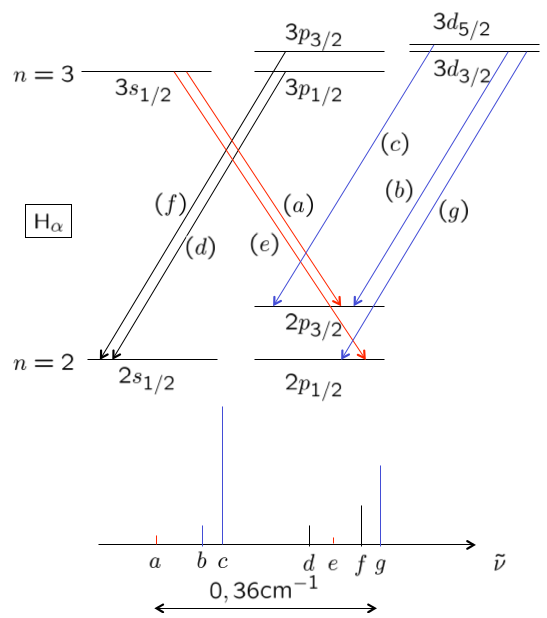
\includegraphics[scale=0.4]{ch1/image8}
	\captionof{figure}{ }
	\end{wrapfigure}
L'élaboration d'une théorie visant à décrire la structure fine vient d'une suprise expérimentale. L'énergie de
l'atome d'hydrogène est donné par
\begin{equation}
E_n = -\frac{Z^2}{2m^2}\ \text{u.a.}
\end{equation}
Cette énergie est indépendante de $m_l$, ce qui implique que $3p_-, 3p_0$ et $3p_+$ ont la même énergie. Ceci
est logique, la différence entre ces niveau est l’orientation de l'orbitale et nous avons bien une invariance
par rotation tant que la symétrie sphérique est conservée. Ceci explique pourquoi l'énergie est indépendante
de $m_l$, on pouvait s'y attendre. L'énergie est également indépendante de $l$ mais on ne peut le deviner : 
c'est une conséquence du potentiel en $1/r$.\\

On se demande combien il y a de raies spectrales entre $n=2$ et $n=3$. Si l'équation de \textsc{Schrödinger} 
est valable, comme les niveaux $n=3$ sont tous dégénérés en énergie, on ne devrai s'attendre qu'à une seule
différence et donc qu'à une seule raie. Or, ce n'est ps ce qui est observé expérimentalement : le niveau
$3d_{3/2}$ n'a pas la même énergie que le niveau $3d_{5/2}$ et ceci résulte de la \textbf{structure fine}. \\

En "observant" la notation spectroscopique, on peut se douter d'une interaction entre $\vec{L}$ et $\vec S$. 
Mais il ne faut pas être trop naïf et penser que tout se résume en $\vec{j}=\vec l +\vec s$ sans quoi 
"\textit{nous aurions fini l'atome d'hydrogène en une demi-heure}". L'appellation \textit{structure fine} 
vient que cet effet est très fin (0.36 cm$^{-1}$), il faut une très bonne résolution pour l’apercevoir.

\section{Effets relativistes et structure fine}
\subsection{L'équation de Dirac}
Soit l'équation de Schrödinger dépendante du temps
\begin{equation}
i \hbar \frac{\partial}{\partial t} \Psi = H \Psi 
\hspace*{3cm} \mbox{lin\'eaire en}~\partial/\partial t !
\end{equation}
\textsc{Dirac} aimait la dépendance temporelle linéaire de cette équation mais il n'aimait pas le 
$p^2/2m$ se cachant dans $T$, soit un terme non-linéaire. Il y avait donc un déséquilibre entre 
le temps et les trois composante d'espace ce qui ne plaisait pas (il y avait de plus pas mal 
d'arguments montrant que Schrödinger ne suffisait pas). Il était nécessaire de tout mettre sur
le même pied
\begin{equation}
(x,y,z,t) = (x_1,x_2,x_3, x_0 \equiv ct) ~\mbox{sur le m\^eme pied}
\end{equation}
Pour se faire, il faut que $H$ soit linéaire en les dérivées d'espace $\partial/\partial x_k$. 
Dirac a su montrer qu'en utilisant une fonction d'onde à quatre composantes, tout se déroulait 
correctement.
\begin{equation}
\Psi = \left(
\begin{array}{c} \Psi_1 \\ \Psi_2 \\ \vdots \\ 
\Psi_4 \end{array}
\right)
\end{equation}
Cette fonction d'onde doit être fonction propre d'un Hamiltonien linéaire en les variable $p$. Il a 
proposé
\begin{equation}
H = c \; \mbox{\boldmath $ \alpha $} \cdot {\bf p}
  + \beta \; mc^2
\end{equation}
Qui est bien linéaire en les variables d'espaces car $p$ apparaît à la place de $p^2$. Pour des raisons
dimensionnelle, il est nécessaire d'effectuer la multiplication par $\alpha$. Notons que, pour garder
la linéarité, $(\alpha^1, \alpha^2, \alpha^3, \beta)$ sont indépendant de $({\bf r},t,{\bf p})$. Grâce
à la présence du $\beta$, on peut également décrire l'antimatière. Écrivons $H\psi = E\psi$
\begin{equation}
(E - c \; \mbox{\boldmath $ \alpha $} \cdot {\bf p}
  - \beta \; mc^2 ) \Psi = 0
\end{equation}
Développons
\begin{equation}
i \hbar \frac{\partial}{\partial t} \Psi =
- i \hbar  c \mbox{\boldmath $ \alpha $} \cdot \mbox{\boldmath $ \nabla $} \Psi +  \beta \; mc^2  \Psi
\end{equation}
Injectons les quatre composante de la fonction d'onde
\begin{equation}
i \hbar \frac{\partial}{\partial t} \Psi_i = -i \hbar c 
\sum_{j=1}^4 \sum_{k=1}^3 \alpha_{ij}^k 
\frac{\partial}{\partial x_k} \Psi_j 
+ \sum_{j=1}^4 \beta_{ij} mc^2 \Psi_j,\qquad (i=1,2,3,4)
\end{equation}
Ceci exprime la variation d'une des quatre composante comme un couplage avec toutes les autres 
composantes. Les termes diagonaux vont se coupler (somme sur $j$) mais il y a une seconde somme
(sur $k$) portant sur les trois composantes de l'impulsion. Le $\alpha^k_{ij}$ est est ainsi une 
matrice. Bien sûr, s'inspirant de Klein-Gordon, Dirac a imposé l'hermiticité de $H$ et fait en sorte
que l'on puisse retomber sur son équation.\\

Au risque de se répéter, nous sommes dans un espace 4D où $\alpha$ est une matrice à quatre 
composantes "cachée" par $\vec \sigma$, les matrices de \textsc{Pauli}. On est alors forcée de 
constater que le spin est "inclus" dans l'équation de \textsc{Dirac}
\begin{equation}
\mbox{\boldmath $ \alpha $} = 
\left( \begin{array}{cc} 0 & \mbox{\boldmath $ \sigma $} \\
\mbox{\boldmath $ \sigma $} & 0 \end{array} \right),\qquad\qquad\qquad
\beta = 
\left( 
\begin{array}{cc} I & 0 \\
0 & - I    \end{array} \right)
\end{equation}

Jusqu'ici, nous ne savons pas comment se comporte une particule chargée munie d'un spin dans un 
champ électromagnétique. Pour en décrire le comportement, il suffit d'effectuer la substitution
$\vec p \to \vec{p}-q\vec{A}$ où $\vec A$ est le potentiel vecteur. On obtient alors
\begin{equation}
H = 
c  \mbox{\boldmath $ \alpha $} \cdot  ( {\bf p} - q {\bf A} )
+ q \Phi + \beta m c^2
\end{equation}
En étudiant les solutions stationnaire de la forme $\Psi ({\bf r},t) = \chi({\bf r}) e^{-iEt/ \hbar}$,
on en tire l'énergie
\begin{equation}
E \chi({\bf r}) =
[ - i \hbar  c \mbox{\boldmath $ \alpha $} \cdot \mbox{\boldmath $ \nabla $}
- c q \mbox{\boldmath $ \alpha $} \cdot {\bf A} + q \Phi + \beta mc^2 ] \chi({\bf r})
\end{equation}
où $\DS \chi ({\bf r}) \equiv \left( \begin{array}{c}
 \psi({\bf r}) \\ \eta({\bf r}) \end{array} \right)$.\\


Considérons un \textbf{champ central} ($\vec{A}=\vec0$). Le potentiel vaut alors $V(r)=q\Phi(r)$ de
sorte que l'on puisse écrire
\begin{equation}
H = 
c  \mbox{\boldmath $ \alpha $} \cdot  {\bf p}
 + \beta m c^2 + V(r)
\end{equation}
L'Hamiltonien non relativiste commutait (impliquant une invariance) avec $\vec{L^2}$ et $L_z$ et de
même pour le spin. La mauvaise nouvelle c'est que ceci n'est plus vérifié ici
\begin{equation}
[H,\vec{L}^2] \neq 0,\qquad\qquad\qquad [H,\vec{S}^2] \neq 0
\end{equation}
Cette non-commutation vient du fait que le $H_{rel}$ dépend du spin via $\alpha$ (qui contient 
$\vec \sigma$, les matrices de \textsc{Pauli}) tandis que la non commutation avec le moment cinétique
orbital vient du fait que $H$ contient $\vec{L}$ et non plu $\vec{L}^2$.\\

Cependant, bonne nouvelle, l'Hamiltonien commute avec le \textbf{moment angulaire total}
\begin{equation}
{\bf J} = {\bf L} + {\bf S} \Rightarrow [ {\bf J}, H ] = 0
\Rightarrow [H, {\bf J}^2] = 0
\end{equation}
Ceci permet de retrouver la relation de commutation $[ H , J_z ] = 0 \Rightarrow ~\mbox{EOC}~ = \{
{\bf J}^2, J_z \}$. Les vecteur/valeurs propres sont donnés par 
\begin{equation}
 \left\{ \begin{array}{l}
{\bf J}^2 \chi_{j,m_j} ({\bf r}) = j(j+1) \hbar^2 \chi_{j,m_j} ({\bf r}) \\
J_z \chi_{j,m_j} ({\bf r}) = m_j \hbar \chi_{j,m_j} ({\bf r}) 
\end{array} \right.
\end{equation}
Les problèmes de Schrödinger viennent d'un couplage mais on se rend ici compte que c'est plus 
fondamental que ça. De même, avec $\vec{J}^2$ on sent venir le couplage \textit{spin-orbite} avec
un facteur $2\vec{L}.\vec{S}$ qui va apparaître.\\

Résumons
\begin{equation}
H = 
c  \mbox{\boldmath $ \alpha $} \cdot  {\bf p}
 + \beta m c^2 + V(r),\qquad\qquad
 \chi ({\bf r}) = \left( \begin{array}{c}
  \psi({\bf r}) \\ \eta({\bf r}) \end{array} \right)
\end{equation}
Avec les relations de commutations
\begin{equation}
[H, {\bf L}^2 ] \neq 0; \hspace*{1cm}  [H, {\bf S}^2 ] \neq 0;,\qquad\qquad\qquad
[H, {\bf J}^2 ] = [H, J_z] = 0
\end{equation}
Décrire un électron avec l'équation de \textsc{Dirac} est compliqué : on va y arriver à l'aide d'une
fonction à quatre composante. Nous allons l'écrire comme quelque chose qui \textit{ressemble} à un
spinneur de rang 2 mais qui n'en est pas un car chacune de ses deux composantes contiennent un peu
de spin \textit{up} et \textit{down}. Il y a donc bien en réalité quatre composantes
\begin{equation}
\chi_{E \kappa m_j} ({\bf r}) =\frac{1}{r} \left( \begin{array}{c}
 {\color{blue} P}_{E \kappa m_j}(r) \xi_{\kappa,m_j}(\theta, \phi) \\ 
 i {\color{red} Q}_{E \kappa m_j} (r)  \xi_{- \kappa, m_j (\theta, \phi)} 
\end{array} \right) 
\end{equation}
Inspectons les valeurs/vecteurs propres
\begin{equation}
\left\{
\begin{array}{l}
{\bf J}^2 \; \chi_{E \kappa m_j} ({\bf r}) = j(j+1) \hbar^2  \; \chi_{E \kappa m_j} ({\bf r})\\
J_z \; \chi_{E \kappa m_j} ({\bf r}) = m_j  \hbar \; \chi_{E \kappa m_j} ({\bf r}) \\
K \; \chi_{E \kappa m_j} ({\bf r}) = \kappa \; \chi_{E \kappa m_j} ({\bf r})
\end{array} \right.
\end{equation}
Où nous avons créer un opérateur $K$ de valeur propre $\kappa = \kappa = -(j+1/2)a$ où $a=\pm1$. 
Afin de comprendre l'intérêt de cet opérateur, considérons le tableau suivant
\begin{equation}
\begin{array}{lcccccc}
  & s_{1/2} & p_{1/2} & p_{3/2} & d_{3/2} & d_{5/2} & f_{5/2}  \\
j & 1/2 & 1/2 & 3/2 & 3/2 & 5/2 & 5/2 \\
l & 0 & 1 & 1 & 2 & 2 & 3 \\
a & +1 & -1 & +1 & -1 & +1 & -1 \\
\kappa & -1 & +1 & -2 & +2 & -3 & +3
\end{array}
\end{equation}
L'intérêt de la valeur propre $\kappa$ est qu'elle permet de désigner de façon unique un électron (
$j$ ou $l$ seul ne suffit pas à complètement caractériser un électron). Elle permettra également de
comprendre l'expression du vecteur propre décrit ci-dessus où l'on voit apparaître $\kappa$ dans la
première composante et $-\kappa$ dans la seconde.

\subsection{Couplage entre petite et grande composantes}
Ré-écrivons notre spinneur de rang 4
\begin{equation}
\chi_{E \kappa m_j} ({\bf r}) =\frac{1}{r} \left( \begin{array}{c}
 P_{E \kappa m_j}(r) \xi_{\kappa,m_j}(\theta, \phi) \\ 
 iQ_{E \kappa m_j} (r)  \xi_{- \kappa, m_j (\theta, \phi)} 
\end{array} \right)
\end{equation}
Ce qu'il faut comprendre, c'est que chacun des six $\kappa$ qui apparaissent est un mélange des 
harmonique. Afin de comprendre pourquoi il existe un tel couplage (on parlera de couplage entre 
la \textit{petite (Q) et la grande (P) composante}) existe, il faut regarder ce qui se cache dans
l'Hamiltonien. Par l'intermédiaire de $\alpha$, nous avons le produit suivant
\begin{equation}
\mbox{\boldmath $ \sigma $} \cdot {\bf p}
\left\{ \frac{F(r)}{r} \xi_{\kappa, m_j} (\theta, \phi) \right\}
= i \hbar \frac{1}{r} \left\{ \frac{dF}{dr} + \frac{\kappa F}{r} \right\}  \xi_{-\kappa, m_j} (\theta, \phi)\}
\end{equation}
Ceci nous renseigne sur l'application de $\vec{\sigma}.\vec{p}$ à une fonction radiale. On peut 
ré-écrire l'application de $H$ sur notre fonction propre
\begin{equation}
\left(
\begin{array}{cc}
mc^2 -E + V  &  -c \hbar \left( \frac{d}{dr} - \frac{\kappa}{r} \right) \\
 c \hbar \left( \frac{d}{dr} + \frac{\kappa}{r} \right) & -mc^2 -E + V 
\end{array} 
\right)
\left(
\begin{array}{c}
P_{E \kappa} (r) \\ Q_{E \kappa} (r) \end{array}
 \right) = 0
\end{equation}
Nous allons nous rendre compte que, dans cet algèbre, $P$ est couplé à $Q$ en développant cette
expression
\begin{equation}
\begin{array}{ll}
\DS\left[  \frac{d}{dr} + \frac{\kappa}{r}   \right] 
{\color{blue} P}_{E \kappa} (r)
&\DS= \frac{E + mc^2 - V(r)}{\hbar c} 
\DS{\color{red} Q}_{E \kappa} (r)\vspace{2mm}\\
\DS\left[  \frac{d}{dr} - \frac{\kappa}{r}   \right] 
{\color{red} Q}_{E \kappa} (r)
&\DS= - \frac{E - mc^2 - V(r)}{\hbar c} 
{\color{blue} P}_{E \kappa} (r)
\end{array}
\end{equation}
Il s'(agit d'une équation différentielle d'ordre 1 en $P$ et $Q$ dont nous avons besoin pour
décrire l'orbitale relativiste. Il existe ainsi bien un couplage radial. Nous avons séparer radialement en supposant une forme (fonction radiale * qqch($\theta,\phi$)) mais ce "quelque chose"
est beaucoup plus compliqué\footnote{Il est nécessaire d'utiliser les coefficients de CG pour écrire
le couplage spin-orbite}.\\
 
Pour s'en rendre compte, considérons un électron $2p$. Si $j=3/2, m_j = -1/2,-3/2,\dots$. Choisissons
$m_j = -1/2$. Déballons nos deux fonctions radiales $P$ et $Q$ (grande et petite composante)
\begin{equation}
\chi_{2p_{{3/2}, -1/2}} ({\bf r}) =\frac{1}{r} \left( \begin{array}{c}
 {\color{blue} P}_{2p_{3/2} }(r) \left(   +\sqrt{\frac{1}{3} } \right) Y_{1,-1} (\theta, \phi)\;  \alpha \\ 
 {\color{blue} P}_{2p_{3/2} }(r) \left(   +\sqrt{\frac{2}{3} } \right) Y_{1,0} (\theta, \phi)\;  \beta \\ 
 i {\color{red} Q}_{2p_{3/2} } (r) \left(   -\sqrt{\frac{3}{5} } \right) Y_{2,-1} (\theta, \phi)\;  \alpha  \\
  i {\color{red} Q}_{2p_{3/2} } (r)  \left(  + \sqrt{\frac{2}{5} } \right) Y_{2,0} (\theta, \phi)\;  \beta \end{array} \right)
\end{equation}
Examinons la première ligne. On retrouve $Y_{1,-1}$ ce qui est cohérent avec un électron $p$ ($l=1$)
et la projection vaut $m_l=1$ car l'égalité $j=l+s$ doit être respectée. Il reste comprendre pourquoi
le spin est \textit{up} (via $\alpha$). Rappelons-nous de la règle de sélection induite par les
coefficients de CG : $m_j=m_l+m_s$. Nous volons construire un état où $m_j = -3/2$. Comme nous avons
un électron $p$, $m_l$ peut valoir -1,0 ou 1. Il faut donc que $m_s=m_j-m_l$. Or comme $m_l=-1$ et 
$m_j=-1/2$ la projection du spin vaut $m_s=1/2$, soit un spin \textit{up}. Le spin étant \textit{down}
pour la seconde ligne, on retrouve bien du $\beta$.\\

La surprise est à la troisième ligne où l'on retrouve l'harmonique sphérique $Y_2$. Ceci vient du fait
que $l$ n'est plus un bon nombre quantique (mais il ne faut pas jeter les harmoniques sphériques pour
autant). La présence de $Y_2$ vient du fait que, dans la définition de $\chi$, $\kappa$ est renvoyé
en $-\kappa$.  Comme l'opérateur change (le signe) de $\kappa$, il va créer un mélange entre 
l'orbitale $p$ et $d$ comme le montre le tableau ci-dessus. Ceci explique la présence des harmoniques
$Y_2$ dans la description d'un électron $p$. Les racines apparaissant ne sont rien d'autres que les
coefficients de CB explicités (à cause du couplage \textit{spin-orbite}).



\subsection{Spectre de Dirac}
	\begin{wrapfigure}[14]{l}{6cm}
	\vspace{-5mm}
	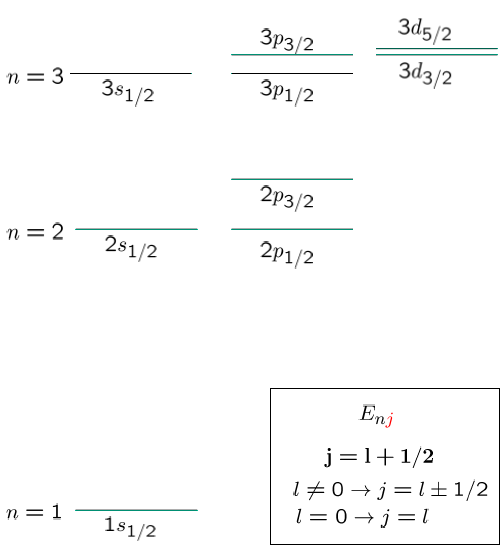
\includegraphics[scale=0.45]{ch1/image82}
	\captionof{figure}{ }
	\end{wrapfigure}
	
Sans surprise, l'énergie de \textsc{Dirac} dépend de $n$, mais aussi du nombre quantique $j$
\begin{equation}
E_{nj}^D = mc^2\times \left[ 1 + 
\left(
\frac{Z \alpha} {n-j-1/2 + [(j+1/2)^2 - Z^2 \alpha^2)^{1/2}}
\right) ^2  \right] ^{-1/2}
\end{equation}
Il s'agit de la solution analytique de \textsc{Dirac}. Afin de faire le lien avec 
\textsc{Schrödinger}, nous allons étudier le comportement de cette solution lorsque $Z\alpha$ n'est
pas trop important ou, autrement dit, lorsque les effets relativistes ne sont pas trop grands. 
Développons alors en puissance de $(Z\alpha)^2$
\begin{equation}
E_{nj}^D = mc^2= mc^2 \left[
1 - \frac{(Z \alpha)^2}{2 n^2} 
- \frac{(Z \alpha)^4}{2n^4} \left(
\frac{n}{j+1/2} - \frac{3}{4} \right) + \ldots \right]
\end{equation}\ \\
Bonne nouvelle : l'énergie relativiste de \textsc{Dirac} n'est autre que $mc^2$ et si on retire cette
énergie, il y a toujours une dépendance en $n$ et $j$. Il est donc possible d'exprimer, en faisant
cette soustraction, l'énergie non relativiste à laquelle s'ajoute des corrections proportionnelles
à l'énergie relativiste\footnote{Pour rappel, le solutions de l'équation de Schrödinger sont 
données par $E_n^{\mbox{NR}} =
- \frac{1}{2} \mu c^2 \frac{(Z \alpha)^2}{n^2} ; \hspace*{1cm}
{\color{red} \alpha = \frac{e^2}{(4 \pi \epsilon_0) 
\hbar c}}$.}
\begin{equation}
E_{n {\color{red} j}} = E^D_{nj} - mc^2 = E_n^{\mbox{NR}} \left[
1 + \frac{(Z \alpha)^2}{n^2} \left(
\frac{n}{{\color{red} j}+1/2} - \frac{3}{4} \right) + \ldots \right]
\end{equation}
Les corrections dépendent évidemment de $j$ et c'est rassurant car si $c\to \infty$, on retrouve
l'énergie non-relativiste qui n'est autre que la valeur propre de l'équation de \textsc{Schrödinger}.


\subsection{Fonctions radiales de Dirac}
Représentons l'orbitale $R$ de \textsc{Dirac}. Soit l'atome de $Hg^{79+}$ où 79 électrons ont été
arrachés de façon à former un système hydrogénoïde. En rouge, la \textit{grande composante} $P$ 
rappelle l'orbitale $2s$. On comprend également la désignation \textit{petite composante} à l'aide
de la courbe en vert représentant $Q$. Si $c\to\infty, Q\to 0$ et la petite composante s'éteint : on
retrouve l'expression de $P$ identique à celle trouvée avec \textsc{Schrödinger}. On peut remarquer
que ces deux composantes ne s'annulent pas au même rayon $r$. La somme des deux composantes ne 
s'annulera donc jamais : disparition de la structure noeudale.\\


On peut voir que l'effet non-relativiste n'est pas négligeable lorsque l'on représente la densité
$NR$ de \textsc{Schrödinger} $D_{n l}(r) = \vert P_{nl}(r) \vert^2 = r^2 R_{nl}(r) ^2$ et la 
densité $R$ de \textsc{Dirac} $D_{n \kappa}(r) = \vert P_{n \kappa}(r) \vert^2
+  \vert Q_{n \kappa}(r) \vert^2$.\\

Comme prévu, la densité ne s'annule jamais. On observe également une contraction de l'onde signifiant
une contraction de l'énergie de liaison. La structure ressemble cependant toujours à celle de 
\textsc{Schrödinger}. Cet effet est également présent dans d'autres orbitales (voir \textit{slide 
45}).


\begin{center}
	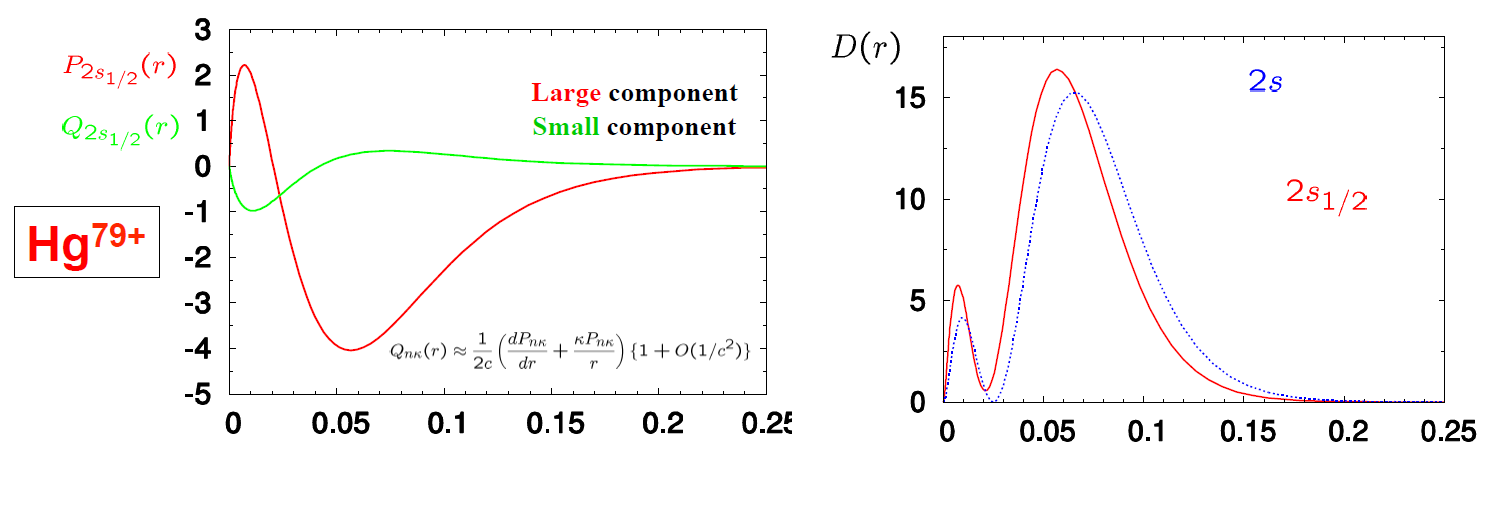
\includegraphics[scale=0.4]{ch1/image9}
	\captionof{figure}{ }
\end{center}

\newpage
\subsection{Limite non relativiste de Dirac}
Il n'est pas possible d'ignorer les résultats obtenu par l'équation de \textsc{Dirac}. Cependant, 
il est possible d'essayer de "mimiquer" le spectre de \textsc{Dirac} en bye-passant la complexité
de son équation. L'idée est d'exprimer l'Hamiltonien de Dirac comme un de Schrödinger additionné à
une perturbation de sorte à pouvoir écrire $H \psi ({\bf r}) = E' \psi ({\bf r})$. \\

Les corrections proposées ci-dessous vont être correctes jusqu'à l'ordre $(v/c)^2$. Considérons un
potentiel central
\begin{equation}
\left\{
\begin{array}{l}
{\bf A } = 0 \\
q \Phi = - e \Phi = V(r) = -\frac{Ze^2}{(4 \pi \epsilon_0) r}
\end{array} \right.
\end{equation}
En mimiquant, on obtient
\begin{equation}
H = \frac{p^2}{2m} + V(r)- \frac{p^4}{8 m^3 {\color{red} c^2}} 
+ \frac{1}{2m^2 {\color{red} c^2}} \frac{1}{r}
  \frac{dV}{dr} {\bf L} \cdot {\bf S} 
 + \frac{\pi \hbar^2}{2 m^2 {\color{red} c^2 } }
  \left( \frac{Ze^2}{4 \pi \epsilon_0} \right) \delta( {\bf r} )
\end{equation}
où $V(r)$ est le potentiel d'interaction des protons, où l'on retruve une correction de \textit{masse
à l'énergie cinétique}
\begin{equation}
H^{\mbox{M}} = - \frac{p^4}{8 m^3 c^2}
\end{equation}
Une correction due à l'interaction \textit{spin-orbite}
\begin{equation}
H^{\mbox{s-o}} = + \frac{1}{2m^2 c^2} \frac{1}{r}
  \frac{dV}{dr} {\bf L} \cdot {\bf S} 
\end{equation}
Et une correction de \textit{Darwin}
\begin{equation}
H^{\mbox{D}} = 
 + \frac{\pi \hbar^2}{2 m^2 c^2 } 
  \left( \frac{Ze^2}{4 \pi \epsilon_0} \right) \delta( {\bf r} )
\end{equation}

La correction la plus parlante est l'interaction spin-orbite venant du fait que \textsc{Dirac} a 
forcé le couplage entre $\vec{L}$ et $\vec S$. Les deux autres corrections sont assez difficile à 
interpréter physiquement et il n'existe pas de consensus sur leur interprétation, nous n'y reviendrons
pas. Notons la signature relativiste de ces corrections via le facteur $1/c^2$. Le \textit{slide 47}
montre l'impact de ces différents corrections au sein de la couche $n=2$. Les \textit{slides 48} à
\textit{53} seront vus en séance d'exercices et ne sont pas repris ici (le but est de dériver
l'expression de l'énergie dû à la structure fine)\footnote{Lire notes personnelles \textit{slide 54}}.



\newpage
\section{Lamb shift (1947)}
\subsection{Levée de la dégénérescence pour $j=1/2$}
La catastrophe (ou beauté) c'est que tout n'est pas prévu par l'équation de \textsc{Dirac}. En 
observant les niveaux $n=2$, \textsc{Lamb} a obtenu trois niveaux et non pas deux comme le 
prévoyait\textsc{Dirac} : il y a une levée de la dégénérescence pour $j=1/2$.\\

	\begin{wrapfigure}[9]{l}{6cm}
	\vspace{-5mm}
	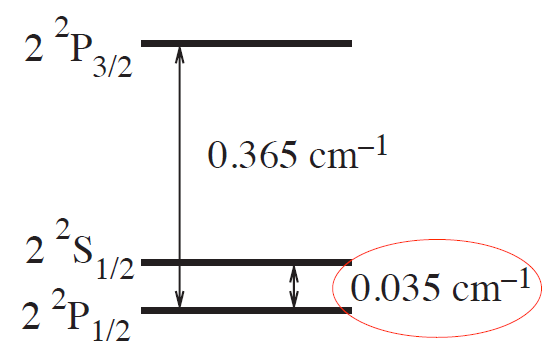
\includegraphics[scale=0.4]{ch1/image10}
	\captionof{figure}{ }
	\end{wrapfigure}
L'énergie dépend non seulement de $j$, mais peut-être bien de $n$ également. Il s'agit d'un effet 
plus fin que la structure fine, mais ce n'est pas la structure \textit{hyperfine} non plus. Il 
s'agit de la première manifestation pour un électron de l'électrodynamique quantique. Cet effet
est causé par les oscillations du vide\footnote{Si l'on admet que le vide sont des petits OH, on 
est forcée de constater que même à température nulle le système vibre encore ($E_v = \hbar\omega/2$.
Il existe donc un champ électromagnétique oscillant dans le fondamental que l'on nomme 
\textit{oscillation du vide du champ EM}.} que \textsc{Dirac} ne prend pas en compte. Or, un 
électron $2s$ ressent ces oscillation différemment qu'un électron $2p$ mais pour calculer ces 
déplacements, il faut se tapper un diagramme de \textsc{Feynman}.\\

L'énergie d'ionisation de l'hydrogène est d'à peu près 110 000 cm$^{-1}$. Ce déplacement de 
\textsc{Lamb} est d'à peu près 0.038 cm$^{-1}$ pour l'hydrogène mais peut atteindre 75 eV pour 
l'uranium.


\section{Structure hyperfine de l'hydrogène}
	\begin{wrapfigure}[14]{r}{7cm}
	\vspace{-5mm}
	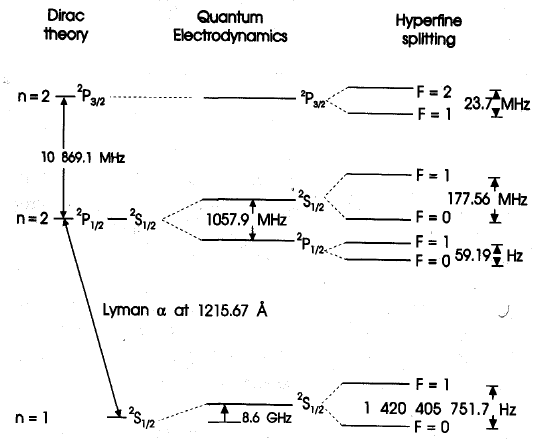
\includegraphics[scale=0.5]{ch1/image11}
	\captionof{figure}{ }
	\end{wrapfigure}
On s'intéresse ici à un effet nucléaire sur la structure électronique. Avec une résolution 
suffisamment fine, on s'aperçoit qu'il n'y a pas deux niveau pour $n=1$ mais quatre. Regardons
l'état fondamental $1s$ en Schrödinger qui devient $^2S_{1/2}$ dans Dirac\footnote{Le 2 en haut à 
gauche représente un \textit{doublet} car l'électron peut être dans deux états de spin (
$S=1/2, m_s =\pm1/2$ : \textit{up} et \textit{down}. Lorsque $S=1, m_s=-1,0,1$ et on parle de triplet.
De même lorsque $S=3/2$, $m_s = \pm 1/2, \pm 3/2$ et on parle de quadruplet, etc. }. \\

Cet effet s'observe même dans un cage de \textsc{Faraday} isolé de tout champ. Cependant, lorsque
l'on place un champ d'induction magnétique le niveau (pour $n=1$) $F=0$ donne un niveau tandis que
$F=1$ se divise en trois niveau (levée de dégénérescence). Il faut trouver quelque chose qui 
préserve l'invariance par rotation mais donnant un couplage\footnote{Si $F=2$, nous aurons 5 
valeurs.}. \\

Ce quelque chose c'est le noyau car le proton ($^1$H) possède un moment angulaire ; un spin noté
$I=1/2$. Il va y avoir un couplage entre $J$ (nature électronique) et $I$ (nature nucléaire)
\begin{equation}
{\bf F} = {\bf J} + {\bf I} \Rightarrow 
F = J+I, J+I-1, \ldots, \vert J-I \vert
\end{equation}
Notons que la théorie de l'électrodynamique quantique justifie un déplacement du fondamental mais
ne met pas en évidence un nouvelle structure. Cette dernière apparaît cependant bien lorsque
l'on \textit{regarde de plus près}. Remarque : $1GHz$ correspond à $\pm 10^{-6}$ eV ce qui n'est 
pas grand chose!\\

Pour chiffrer ces effets, on utilise le \textit{moment magnétique de spin $\mu_I$}, le 
\textit{magnéton de Bohr} $\mu_B$ et le \textit{magnéton nucléaire} $\mu_N$
\begin{equation}
\mbox{\boldmath $ \mu $}_I = g_I \mu_N {\bf I}/ \hbar,\qquad\qquad
\mu_B = \frac{e \hbar}{2m_e},\qquad\qquad
\mu_N = \frac{e \hbar}{2M_p} = \frac{m_e}{M_p} \mu_B
\end{equation}
Le moment nucléaire est colinéaire au moment magnétique : le rapport $\mu_N/\mu_B$ vaut à peu près
1836. La définition de $\vec F$ crée évidemment un nouvel \textsc{ecoc}.

\subsection{État fondamental $1s_{1/2}$}
Considérons l'interaction hyperfine dipolaire magnétique (M1)
\begin{equation}
H = H^0 + H^{M1}
\end{equation}
Il existe des interactions avec le spin de l'électron. Dans l'état $1s$, nous avons 
${\bf J} = {\bf L} + {\bf S} = {\bf S}$. En définissant $\mbox{\boldmath $ \mu $}_S = -g_S \mu_B {\bf
S}/ \hbar$, on peut écrire un Hamiltonien décrivant cette interaction
\begin{equation}
H^{M1}_{\mbox{spin}} = - \mbox{\boldmath $ \mu $}_S \cdot 
{\bf B} = 2 \mu_B {\bf S} \cdot {\bf B} / \hbar
\end{equation}
Pour l'obtenir on travaillera avec le potentiel vecteur ${\bf A} ({\bf r}) = - \frac{\mu_0}{4 \pi}
\left[ \mbox{\boldmath $ \mu $}_I \times \mbox{\boldmath $ \nabla $} \left( \frac{1}{r} \right)
\right]$ avec lequel il est possible d'en tirer ${\bf B} = \mbox{\boldmath $ \nabla $} \times {\bf A}
= -\frac{\mu_0}{4 \pi} \left[\mbox{\boldmath $ \mu $}_I \nabla^2 \left( \frac{1}{r}  \right)
 - \mbox{\boldmath $ \nabla $} ( \mbox{\boldmath $ \mu $}_I \cdot \mbox{\boldmath $ \nabla $} )
\frac{1}{r} \right]$. Malheureusement, nous n'avons pas le temps de nous attarder la dessus.\\

Notons cependant que via l'\textit{interaction de contact de Fermi} ($m=0$), nous pouvons écrire
que
\begin{equation}
\nabla^2 \left( \frac{1}{r} \right)  
= -4 \pi {\color{red} \delta ({\bf r})  } \neq 0 
\hspace*{1cm}
{\color{red} ~\mbox{ssi}~l=0  }
\hspace*{1cm} (R_{nl} (r) \sim r^l )
\end{equation}
Il s'agit de l'équation de \textsc{Poisson}.On peut ré-écrire notre Hamiltonien
\begin{equation}
H^{M1}_{\mbox{spin}}  =  
\frac{\mu_0}{4 \pi} \frac{2}{\hbar^2} 
g_I \mu_B \mu_N 
\frac{8 \pi}{3} 
{\color{red}  \delta( {\bf r})}
\;  {\bf S} \cdot {\bf I}
\end{equation}
On peut lier cette relation avec la correction de \textsc{Darwin} qui contenait un $\delta(\vec{r})$,
il s'agit d'une première justification de cette expression.


\subsection{État $ns_{1/2}$}
Nous avons précédemment établi 
\begin{equation}
H^{M1}_{\mbox{spin}}  =  \frac{\mu_0}{4 \pi} \frac{2}{\hbar^2} g_I \mu_B \mu_N \frac{8 \pi}{3} \delta( {\bf r})
\;  {\bf S} \cdot {\bf I}
\end{equation}
Dans notre cas $l = 0 \Rightarrow {\bf F} = {\bf J} + {\bf I} =  {\bf S} + {\bf I}$ et donc 
${\bf S} \cdot {\bf I} = \frac{1}{2} ({\bf F}^2 - {\bf I}^2 - {\bf S}^2)$.\\

Nous pouvons écrire le \textit{ket} suivant, où nous avons couplé $S$ et $I$ pour donner $F$
\begin{equation}
\vert ns_{1/2}IFM_F \rangle=  \sum_{(m_j=m_s),M_I}
\vert ns_{1/2}m_s I M_I \rangle 
\langle ns_{1/2}m_s I M_I 
\vert ns_{1/2}IFM_F \rangle  
\end{equation}
Ce qui nous permet de calculer l'énergie moyenne
\begin{equation}
\Delta E_{\color{red} F} = \langle ns_{1/2}IFM_F \vert H^{M1}_{\mbox{spin}}
\vert ns_{1/2}IFM_F \rangle  = \frac{A}{2} [ {\color{red} F}({\color{red} F}+1) 
- I(I+1) - \frac{1}{2}(\frac{1}{2}+1)]
\end{equation}
où $\DS A =
\frac{\mu_0}{4 \pi} 2  
g_I \mu_B \mu_N \frac{8 \pi}{3} 
 {\color{red} \langle \delta( {\bf r})  \rangle }$. Calculons la valeur moyenne du delta de
\textsc{Dirac}
\begin{equation}
\langle \delta( {\bf r}) \rangle = \int \vert \psi_{n00} (r) \vert^2
\delta( {\bf r} ) d{\bf r} = \vert \psi_{n00} (0) \vert^2 = 
\frac{{\color{red} Z^3}}{\pi a_\mu^3 {\color{red} n^3}}
\end{equation}
Cette valeur moyenne n'est pas nulle grâce à faut qu'il n'y a pas d'annulation en $r=0$ pour les
électrons $s$. On en tire
\begin{equation}
A =
\frac{\mu_0}{4 \pi}  \frac{16 \pi}{3} g_I \mu_B \mu_N  
\frac{Z^3}{\pi a_\mu^3 n^3}
\end{equation}


\subsection{Levée de dégénérescence pour $1s_{1/2}$}
Une image vaut mieux qu'un long discours

\begin{center}
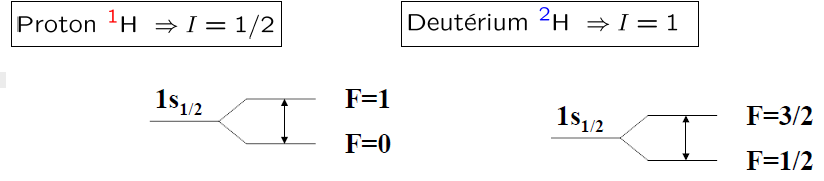
\includegraphics[scale=0.45]{ch1/image12}
\captionof{figure}{Notons pour le $^1$H le bon accord théorie expérience : $v_{th} \approx 1420$ MHz, 
$\nu_{exp} = 1420405751.800$ Hz. Il s'agit de la raie à $\lambda=21$ cm.}
\end{center}






\subsection{Interaction hyperfine électrique quadrupolaire}
En plus de l'interaction hyperfine dipolaire magnétique $M1$ dont nous avons discuté ci-dessus, il
existe l'interaction hyperfine électrique quadrupolaire $E2$\footnote{Voir cours de \textit{Physique
nucléaire.}}
\begin{equation}
H = H^0 + H^{M1} + H^{E2}
\end{equation}
Nous avions déjà énoncé le moment magnétique de spin $\mbox{\boldmath $ \mu $}_I = g_I \mu_N {\bf I}/
\hbar$. Définissons maintenant le \textit{moment quadrupolaire électrique du noyau}
\begin{equation}
Q = \langle I, M_I=I \vert Q_{zz} \vert I, M_I=I \rangle
= \langle I, M_I=I \vert \sum_p (3 z^2_p - r^2_p)  \vert I, M_I=I \rangle
\end{equation}
Si l'on effectue le changement de variable $z=r\cos\theta$, on retrouve la partie radiale de 
$Y_{20}$. La valeur moyenne de ce moment angulaire se calcule alors
\begin{equation}
Q_{20} = sum_p r_p^2 Y_{20}(\Omega_p)
\end{equation}
où l'on somme sur tous les protons\footnote{Il faudrait expliciter, je n'ai pas tout compris. Il 
faut les notes du tableau!}. La composante $z$ peut être calculée par deux fonctions
nucléaires. En fonction du signe de $Q$ trois cas peuvent se présenter (soit la distance de charge 
nucléaire) : sphérique $(Q=0)$, prolate ($Q>0$) et oblate ($Q<0$). Si $I=0$ ou $I=1/2$, il en vient
que $Q=0$. Par exemple, $Q(^2\mbox{H}) = 0.0028~\mbox{barns} = 0.0028~10^{-24}~\mbox{cm}^{2}$.



\section{Largeurs de raies}
\subsection{Largeur naturelle}

	\begin{wrapfigure}[15]{r}{5cm}
	\vspace{-5mm}
	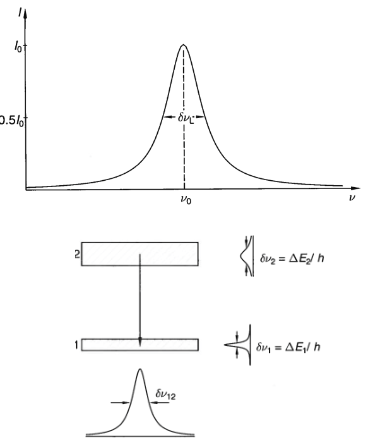
\includegraphics[scale=0.5]{ch1/image13}
	\captionof{figure}{ }
	\end{wrapfigure}
	
Même si \textsc{Schrödinger}, \textsc{Dirac}, \dots prévoient tous des niveaux bien distincts, ce 
n'est pas le cas en pratique (à cause des incertitudes sur les niveaux). Il peut donc pour une 
transition entre deux niveau, émettre des photons de différentes énergies (à cause des incertitudes
sur les deux niveaux). On peut montrer que la largeur naturelle (qui concerne même le fondamental et
qui donc empêche d'avoir des raies parfaitement piquées) est un profil lorentzien, ici exprimé 
en fonction de l'intensité
\begin{equation}
I(\nu) = I_0 \; \frac{ (\gamma / 4\pi )^2}
{ (\nu - \nu_0 )^2 + (\gamma / 4\pi )^2 }
\end{equation}
On peut en définir la largeur à mi-hauteur $\delta \nu_L = \gamma / 2 \pi$. Ce coefficient $\gamma$
n'est en réalité rien d'autre que le coefficient d'\textsc{Einstein} d'émission spontanée
\begin{equation}
\gamma = A_{21} = 1 / \tau_2 \rightarrow 
\delta \nu_L = \frac{1}{2 \pi \tau_2}
\end{equation}
ici de $2\to1$. Comme mentionné ci-dessus, il faut tenir compte de l'incertitude des deux niveaux. 
La largeur à mi-hauteur s'écrit alors
\begin{equation}
\delta\nu_{12}=\delta\nu_1+\delta\nu_2 = \frac{1}{2\pi}\left(\frac{1}{2\pi\tau_2}+\frac{1}{2\pi\tau_2}
\right)
\end{equation}



\subsection{Élargissement par pression}
Comme on l'a déjà dit, même avec \textsc{Dirac, Schrödinger}, \dots où on croit avoir une raie bien
pure il y aura un élargissement, notamment par pression. La forme mathématique est équivalente, il
s'agit d'une lorentzienne
\begin{equation}
I(\nu) = I_0 \; \frac{ (w/2 )^2}
{ (\nu - \nu_0 - d )^2 + (w/2 )^2 }
\end{equation}
Sauf qu'ici, la largeur à mi-hauteur est liée à $w$ qui vaut
\begin{equation}
w =  \frac{1}{ 2 \pi t_0}
\end{equation}
où l'on voit apparaître $t_0$, le temps moyen entre collisions. A pression nulle, chaque particule 
possède un libre parcours moyen infini. Pour se débarrasser de cet effet on effectue les manipulations
à différentes mesures et on essaye d'extrapoler à pression nulle afin d'avoir un signal "idéal". Les
manipulations d'atomes froids sont aussi courants dans ce domaine.


\subsection{Élargissement Doppler}
Hélas il n'y avait pas que cet effet et il y a bien pire : l'effet \textsc{Doppler}
\begin{equation}
\omega = \left(
\frac{1 \mp v/c}{1 \pm v/c} \right) ^{1/2} \omega_0
\end{equation}
La fréquence que l'on voit dans une raie n'est propre que s'il n'y a pas ni mouvement, ni dynamique
entre la source émettrice et l'observateur (ou l'inverse). La fréquence apparente n'est pas la 
fréquence propre. Développons en série
\begin{equation}
\omega - \omega_0 = \mp \frac{v}{c} \omega_0
+ \frac{1}{2} \frac{v^2}{c^2} \omega_0 + \ldots
\end{equation}
Au premier ordre
\begin{equation}
\omega = \omega_0 \left( 1 \mp \frac{v}{c} \right),\qquad\qquad\qquad
\lambda = \lambda_0 \left( 1 \pm \frac{v}{c} \right)
\end{equation}
On peut alors avoir un \textit{red-shift} $\omega = \omega_0 \left( 1 {\color{red} - } 
\frac{v}{c} \right)$ ou un \textit{blue-shift} $\omega = \omega_0 \left( 1 {\color{blue} + } 
\frac{v}{c} \right)$.\\

C'est lorsque une source d'émission s'approchant de l'observateur à vitesse $v_x$ que l'on parle
de décalage vers le bleu. Celui-ci est donné par
\begin{equation}
- \frac{\Delta \lambda }{\lambda_0} =
\frac{\Delta \nu}{\nu_0} = \frac{ \nu - \nu_0 }{\nu_0}  
= \frac{v_x}{c}
\end{equation}
La distribution de Maxwell des vitesses des atomes nous permet, à l'équilibre et à la température
$T$, de connaître la fraction d'atomes ayant une vitesses comprises entre $v_x$ et $v_x+dv_x$
\begin{equation}
dN(v_x) = N_0 \exp (-M v_x^2 /2kT) \; dv_x
\end{equation}
Avoir connaissance de la vitesse est important : l'effet \textsc{Doppler} est nul pour une source 
se déplaçant orthogonalement à l'observateur, mais est colossal lorsqu'une particule se rapproche
vers l'observateur.\\

La profil est cette fois-ci gaussien
\begin{equation}
I(\nu) =  I_0 \; e^{-x^2}~~\mbox{avec}~~
x = 2 \sqrt{\ln 2} \; \frac{\nu_0 - \nu}{\delta \nu_D}
\end{equation}
La largeur à mi-hauteur (\textsc{fwhm}) est donnée par
\begin{equation}
\delta \nu_D = 
2 \sqrt{\ln 2} \; \frac{\nu_0}{c} 
 \sqrt {\frac{2 k{\color{red} T}}
{ {\color{red} M} }}
\end{equation}
Cette largeur est inversement proportionnelle à la racine de la masse. Si la masse est grande, pour
une même énergie, la particule ne se déplacera pas de la même façon. La largeur \textsc{Doppler} sera
donc suffisamment mince pour de gros noyaux. On s'intéresse ici également aux atomes froid, dont le
but est d'immobiliser un atome. S'il est piéger, il ne subit plus d'effet de pression et il n'y a 
pas d'effet \textsc{Doppler}.\\

	\begin{wrapfigure}[8]{r}{5.7cm}
	\vspace{-5mm}
	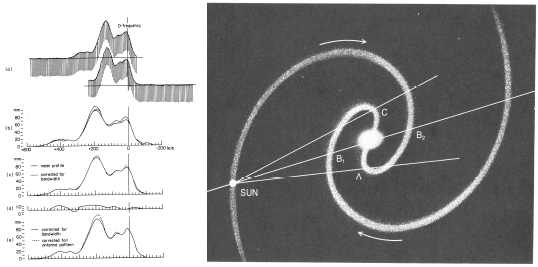
\includegraphics[scale=0.4]{ch1/image14}
	\captionof{figure}{ }
	\end{wrapfigure}
Cet effet peut paraître anodin, mais on l'a rencontré dans l'étude
des systèmes binaires (décale une raie parfois dans un sens, parfois dans l'autre). Autre exemple,
\textsc{Ewen} et \textsc{Purcell} n'ont pas observé une raie bien étroite de 21cm en observant la
\textit{Milkyway}, mais une raie avec une certaine largeur. En pointant sur le centre de la 
galaxie, certaines étoiles se rapprochent et d'autres s'éloignent : shift. C'est ce qui a permis de
modéliser la forme de notre galaxie.


\subsection{Comparaison des profils Doppler et Lorentzien, convolution et profil de Voigt}
Lorsque les deux effets sont présents en même temps, il se produit une convolution entre ces deux effets. Ceci donne un \textit{profil de} \textsc{Voigt}
\begin{equation}
I(x) = \mbox{cste} \; 
\int_{-\infty}^\infty 
\frac{e^{-y^2}}{(x-y)^2 + a^2} dy
\end{equation}
où $\DS x = 2 \sqrt{ \ln 2} \; \;
\frac{\nu_0 - \nu}{\delta \nu_D}$ et $\DS a =  \sqrt{ \ln 2} \; \; 
\frac{\delta \nu_L}{\delta \nu_D}$.